\documentclass[10pt,a4paper,portrait]{article}

\usepackage[utf8]{inputenc}
\usepackage[a4paper,portrait,margin=0.68in,top=0.65in,bottom=0.68in]{geometry}
\usepackage{tikz}
\usetikzlibrary{shapes,arrows,positioning,calc,fit,backgrounds}
\usepackage{xcolor}
\usepackage{lmodern}
\usepackage{booktabs}
\usepackage{tabularx}
\usepackage{enumitem}
\usepackage{titlesec}
\usepackage{fancyhdr}
\usepackage{hyperref}
\usepackage{microtype}

% =========================================================
% Palette & Styling
% =========================================================
\definecolor{primary}{RGB}{24, 43, 73}        % Deep clean navy
\definecolor{secondary}{RGB}{14, 116, 144}   % Teal accent
\definecolor{darkslate}{RGB}{30, 41, 59}     % Normal text color
\definecolor{boxbg}{RGB}{248, 250, 252}      % Soft light box
\definecolor{bordergray}{RGB}{226, 232, 240} % Light border

% Terminal Color Scheme: Modern Light Grey Theme
\definecolor{termbg}{RGB}{246, 248, 250}     % Light grey terminal body
\definecolor{termbar}{RGB}{229, 231, 235}    % Medium light grey title bar
\definecolor{termborder}{RGB}{209, 213, 219} % Crisp border line
\definecolor{termtext}{RGB}{31, 41, 55}      % Dark charcoal text
\definecolor{termuser}{RGB}{22, 101, 52}     % Dark green for user
\definecolor{termhost}{RGB}{21, 128, 61}     % Green for host
\definecolor{termpath}{RGB}{29, 78, 216}     % Blue for directory path
\definecolor{termcmd}{RGB}{17, 24, 39}       % Bold black for commands
\definecolor{termout}{RGB}{55, 65, 81}       % Clear dark grey for outputs
\definecolor{termdir}{RGB}{37, 99, 235}      % Blue for directories
\definecolor{termfile}{RGB}{31, 41, 55}      % Dark for regular files
\definecolor{termhidden}{RGB}{107, 114, 128} % Muted grey for hidden files
\definecolor{termsize}{RGB}{180, 83, 9}      % Amber for sizes
\definecolor{termperm}{RGB}{79, 70, 229}     % Indigo for permissions

% =========================================================
% Section Headings
% =========================================================
\titleformat{\section}
  {\color{primary}\large\bfseries\sffamily}
  {\thesection.}{0.5em}{}
\titlespacing*{\section}{0pt}{8pt}{3pt}

\titleformat{\subsection}
  {\color{secondary}\normalsize\bfseries\sffamily}
  {\thesubsection}{0.5em}{}
\titlespacing*{\subsection}{0pt}{6pt}{2pt}

% =========================================================
% Headers and Footers
% =========================================================
\pagestyle{fancy}
\fancyhf{}
\renewcommand{\headrulewidth}{0.4pt}
\renewcommand{\footrulewidth}{0pt}
\fancyhead[L]{\small\sffamily\color{darkslate} Operating Systems Lab}
\fancyhead[R]{\small\sffamily\color{darkslate} Lab Report: Linux Navigation}
\fancyfoot{}

% First page style: no header at top, no footer at bottom
\fancypagestyle{firstpage}{%
  \fancyhf{}
  \renewcommand{\headrulewidth}{0pt}
  \renewcommand{\footrulewidth}{0pt}
}

% =========================================================
% Terminal Window Macro (Light Grey with Crisp Edges)
% =========================================================
\newcommand{\termprompt}[1][\textasciitilde]{%
  \textbf{\textcolor{termuser}{ratul}}\textcolor{termtext}{@}\textbf{\textcolor{termhost}{firefly}}\textcolor{termtext}{:}\textbf{\textcolor{termpath}{#1}}\textcolor{termcmd}{\$}\ %
}

\newcommand{\terminalwindow}[3][\linewidth]{%
\begin{center}
\begin{tikzpicture}
  % 1. Terminal text on main layer
  \node[
      text=termtext,
      font=\ttfamily\fontsize{7.2}{9.2}\selectfont,
      align=left,
      text width=\dimexpr#1-0.95cm\relax,
      inner xsep=7pt,
      inner ysep=7pt,
      anchor=north west
  ] (body) at (0.32cm, -0.56cm) {#3};

  % Coordinates
  \coordinate (topleft) at (0, 0);
  \coordinate (bottomright) at ($(body.south -| #1, 0) + (0, -6pt)$);
  \coordinate (titlecenter) at ($0.5*(topleft) + 0.5*(#1, 0) + (0, -0.28cm)$);

  % 2. Background and Title bar on background layer
  \begin{scope}[on background layer]
    % Light grey terminal body
    \fill[termbg, rounded corners=6pt] (topleft) rectangle (bottomright);

    % Title bar (clipped to match rounded top corners)
    \begin{scope}
      \clip[rounded corners=6pt] (topleft) rectangle (bottomright);
      \fill[termbar] (topleft) rectangle (#1, -0.56cm);
      \draw[termborder, line width=0.5pt] (0, -0.56cm) -- (#1, -0.56cm);
    \end{scope}

    % Continuous outer border (smooth, no distortion)
    \draw[termborder, line width=0.6pt, rounded corners=6pt] (topleft) rectangle (bottomright);
  \end{scope}

  % 3. Window control dots
  \fill[red!80!black] (0.36cm, -0.28cm) circle (0.07cm);
  \fill[yellow!80!black] (0.63cm, -0.28cm) circle (0.07cm);
  \fill[green!75!black] (0.90cm, -0.28cm) circle (0.07cm);

  % 4. Centered terminal title
  \node[
      text=gray!40!black,
      font=\sffamily\bfseries\fontsize{7.2}{8}\selectfont,
      anchor=center
  ] at (titlecenter) {#2};
\end{tikzpicture}
\end{center}
\vspace{-6pt}
}

\newcommand{\cmd}[1]{\texttt{\textbf{#1}}}

\begin{document}
\thispagestyle{firstpage}

% =========================================================
% Title: Only Experiment Title at the Top
% =========================================================
\begin{center}
  {\Large\bfseries\sffamily\color{primary} Experiment Title: Practice of Basic Linux Terminal Commands}\\[3pt]
  {\normalsize\sffamily\textbf{Topic:} File and Directory Navigation in Linux Terminal}
\end{center}
\vspace{-4pt}

% =========================================================
% 1. Objective
% =========================================================
\section{Objective}
The objective of this lab is to learn how to use the Linux terminal for daily file and directory tasks. By completing this experiment, we aim to:
\begin{itemize}[noitemsep,topsep=1pt,leftmargin=1.2em]
  \item Learn who is currently logged in using \cmd{whoami} and find our current location using \cmd{pwd}.
  \item Move between folders easily using \cmd{cd} and return home using \cmd{cd \textasciitilde}.
  \item View regular files, hidden files, and file details (like size and permissions) using \cmd{ls} and its flags (\cmd{-l}, \cmd{-a}, \cmd{-lh}, \cmd{-la}).
\end{itemize}

% =========================================================
% 2. Equipment / Software Requirements
% =========================================================
\section{Equipment / Software Requirements}
\vspace{-2pt}
\begin{table}[h!]
\centering\footnotesize
\renewcommand{\arraystretch}{1.08}
\begin{tabularx}{\linewidth}{lXlX}
\toprule
\textbf{Item} & \textbf{Details} & \textbf{Item} & \textbf{Details} \\
\midrule
\textbf{Operating System} & Linux (NixOS 26.11, Kernel 6.12) & \textbf{Host Machine} & \texttt{firefly} \\
\textbf{User Account} & \texttt{ratul} & \textbf{Command Shell} & GNU Bash 5.2 / Zsh \\
\textbf{Terminal Emulator} & Linux Terminal (Kitty / Ghostty) & \textbf{Core Tools} & GNU Coreutils (\texttt{ls}, \texttt{pwd}, \texttt{whoami}) \\
\bottomrule
\end{tabularx}
\end{table}
\vspace{-8pt}

% =========================================================
% 3. Theoretical Background
% =========================================================
\section{Theoretical Background}
In Linux, all files and folders (called directories) are organized in a single upside-down tree structure. The very top folder is called the root folder, written as \cmd{/}. 

When a user logs in, they start in their personal home directory (\texttt{/home/ratul}), which is also written as a tilde (\cmd{\textasciitilde}). The terminal allows us to move around this tree and manage files using simple text commands.

\subsection{Commands Practiced in This Lab}
\vspace{-2pt}
\begin{table}[h!]
\centering\footnotesize
\renewcommand{\arraystretch}{1.06}
\begin{tabularx}{\linewidth}{llp{5.4cm}X}
\toprule
\textbf{Command} & \textbf{Syntax} & \textbf{Simple Meaning / Purpose} & \textbf{Example} \\
\midrule
\cmd{whoami} & \texttt{whoami} & Prints the username of the logged-in user. & \texttt{whoami} \\
\cmd{pwd} & \texttt{pwd} & Prints the full path of the current folder you are inside. & \texttt{pwd} \\
\cmd{cd} & \texttt{cd [folder]} & Moves into the specified folder. & \texttt{cd lab\_demo} \\
\cmd{cd \textasciitilde} & \texttt{cd \textasciitilde} & Takes you straight back to your home folder. & \texttt{cd \textasciitilde} \\
\cmd{ls} & \texttt{ls} & Lists the visible files and folders in the current folder. & \texttt{ls} \\
\cmd{ls -l} & \texttt{ls -l} & Long listing: shows file details (permissions, size, date). & \texttt{ls -l} \\
\cmd{ls -a} & \texttt{ls -a} & Shows \textit{all} files, including hidden files starting with a dot (\texttt{.}). & \texttt{ls -a} \\
\cmd{ls -lh} & \texttt{ls -lh} & Shows file details with easy-to-read sizes (K, M, G). & \texttt{ls -lh} \\
\cmd{ls -la} & \texttt{ls -la} & Shows all files (including hidden ones) with full details. & \texttt{ls -la} \\
\bottomrule
\end{tabularx}
\end{table}
\vspace{-6pt}

\subsection{Understanding File Details (\texttt{ls -l})}
When we run \cmd{ls -l}, Linux shows seven pieces of information for each file:
\vspace{-2pt}
\begin{table}[h!]
\centering\footnotesize
\renewcommand{\arraystretch}{1.06}
\begin{tabularx}{\linewidth}{p{3.2cm}X}
\toprule
\textbf{Field} & \textbf{Simple Explanation} \\
\midrule
\textbf{1. File Type \& Permissions} & 10 letters (e.g., \texttt{-rw-r--r--}): the first letter shows if it is a normal file (\texttt{-}) or a directory (\texttt{d}). The next 9 letters show read (\texttt{r}), write (\texttt{w}), and execute (\texttt{x}) rights for owner, group, and others. \\
\textbf{2. Links} & How many directory links point to this file. \\
\textbf{3. Owner \& Group} & Who owns the file (\texttt{ratul}) and which group it belongs to (\texttt{users}). \\
\textbf{4. File Size} & How big the file is in bytes (or in KB/MB when using \cmd{-h}). \\
\textbf{5. Date \& Time} & The day and time the file was last edited. \\
\textbf{6. File Name} & The name of the file or folder. \\
\bottomrule
\end{tabularx}
\end{table}

\newpage

% =========================================================
% 4. Demo Folder Setup
% =========================================================
\section{Equipment / Demo Directory Setup}
To practice these commands, we set up a demo folder called \cmd{lab\_demo} inside \texttt{/home/ratul}. It contains subfolders, regular documents, a script, and hidden files:

\begin{center}
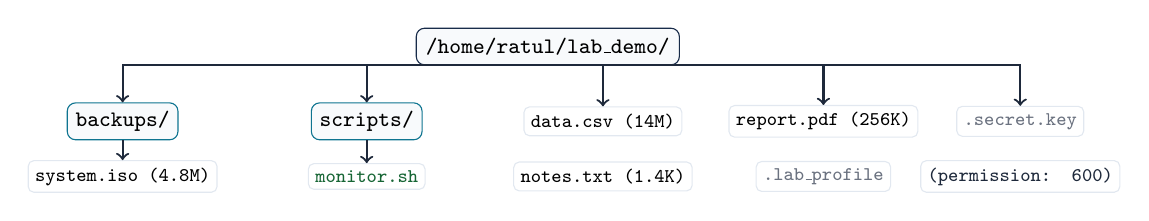
\begin{tikzpicture}[
  x=1cm, y=1cm,
  dirbox/.style={draw=primary, fill=boxbg, rounded corners=3pt, font=\ttfamily\footnotesize\bfseries, inner sep=3.5pt},
  subbox/.style={draw=secondary, fill=boxbg, rounded corners=3pt, font=\ttfamily\footnotesize\bfseries, inner sep=3pt},
  filebox/.style={draw=bordergray, fill=white, rounded corners=2pt, font=\ttfamily\scriptsize, inner sep=2.5pt},
  hiddenbox/.style={draw=bordergray, fill=white, rounded corners=2pt, font=\ttfamily\scriptsize, text=termhidden, inner sep=2.5pt}
]
  % Root node
  \node[dirbox] (root) at (0, 0) {/home/ratul/lab\_demo/};

  % Branches
  \node[subbox] (bdir) at (-5.4, -0.95) {backups/};
  \node[filebox] (iso)  at (-5.4, -1.65) {system.iso (4.8M)};

  \node[subbox] (sdir) at (-2.3, -0.95) {scripts/};
  \node[filebox] (sh)   at (-2.3, -1.65) {\textcolor{termuser}{\textbf{monitor.sh}}};

  \node[filebox] (f1)   at (0.7, -0.95) {data.csv (14M)};
  \node[filebox] (f2)   at (0.7, -1.65) {notes.txt (1.4K)};

  \node[filebox] (f3)   at (3.5, -0.95) {report.pdf (256K)};
  \node[hiddenbox] (h1) at (3.5, -1.65) {.lab\_profile};

  \node[hiddenbox] (h2) at (6.0, -0.95) {.secret.key};
  \node[filebox] (note) at (6.0, -1.65) {\textcolor{darkslate}{(permission: 600)}};

  % Arrows
  \draw[->, thick, darkslate] (root.south) -| (bdir.north);
  \draw[->, thick, darkslate] (bdir.south) -- (iso.north);
  \draw[->, thick, darkslate] (root.south) -| (sdir.north);
  \draw[->, thick, darkslate] (sdir.south) -- (sh.north);
  \draw[->, thick, darkslate] (root.south) -| (f1.north);
  \draw[->, thick, darkslate] (root.south) -| (f3.north);
  \draw[->, thick, darkslate] (root.south) -| (h2.north);
\end{tikzpicture}
\end{center}
\vspace{-8pt}

% =========================================================
% 5. Procedure / Steps
% =========================================================
\section{Procedure / Steps}
We ran the commands in order through the following simple steps:
\begin{enumerate}[noitemsep,topsep=1pt,leftmargin=1.4em]
  \item Checked current user with \cmd{whoami} and checked current folder with \cmd{pwd}.
  \item Listed folders inside our home directory using \cmd{ls}.
  \item Entered the demo directory using \cmd{cd lab\_demo} and confirmed the new location with \cmd{pwd}.
  \item Listed regular files using \cmd{ls}.
  \item Listed all files including hidden files using \cmd{ls -a}.
  \item Checked full file details and byte sizes using \cmd{ls -l}.
  \item Checked easy-to-read file sizes (KB, MB) using \cmd{ls -lh}.
  \item Checked all files (including hidden) with complete details using \cmd{ls -la}.
  \item Returned directly back to the home directory using \cmd{cd \textasciitilde} and verified with \cmd{pwd}.
\end{enumerate}

% =========================================================
% 6. Result / Output Demonstration (Session 1)
% =========================================================
\section{Result / Output Demonstration}
All commands were executed in the terminal under user \texttt{ratul} on machine \texttt{firefly}.

\subsection{Session 1: Finding Our Location, Moving Folders, and Listing Files}

\terminalwindow{ratul@firefly: \textasciitilde\ \textemdash\ bash}{
% Command 1: whoami
\termprompt[\textasciitilde]\textbf{\textcolor{termcmd}{whoami}}

\textcolor{termout}{ratul}

\vspace{0.14cm}
% Command 2: pwd
\termprompt[\textasciitilde]\textbf{\textcolor{termcmd}{pwd}}

\textcolor{termout}{/home/ratul}

\vspace{0.14cm}
% Command 3: ls in home
\termprompt[\textasciitilde]\textbf{\textcolor{termcmd}{ls}}

\textcolor{termdir}{\textbf{Desktop}}\ \ \ \ \textcolor{termdir}{\textbf{Documents}}\ \ \ \ \textcolor{termdir}{\textbf{Downloads}}\ \ \ \ \textcolor{termdir}{\textbf{lab\_demo}}\ \ \ \ \textcolor{termdir}{\textbf{Music}}\ \ \ \ \textcolor{termdir}{\textbf{Pictures}}\ \ \ \ \textcolor{termdir}{\textbf{Videos}}

\vspace{0.14cm}
% Command 4: cd lab_demo
\termprompt[\textasciitilde]\textbf{\textcolor{termcmd}{cd lab\_demo}}

\vspace{0.08cm}
% Command 5: pwd inside demo
\termprompt[\textasciitilde/lab\_demo]\textbf{\textcolor{termcmd}{pwd}}

\textcolor{termout}{/home/ratul/lab\_demo}

\vspace{0.14cm}
% Command 6: ls inside demo
\termprompt[\textasciitilde/lab\_demo]\textbf{\textcolor{termcmd}{ls}}

\textcolor{termdir}{\textbf{backups}}\ \ \ \ \textcolor{termfile}{data.csv}\ \ \ \ \textcolor{termfile}{notes.txt}\ \ \ \ \textcolor{termfile}{report.pdf}\ \ \ \ \textcolor{termdir}{\textbf{scripts}}

\vspace{0.14cm}
% Command 7: ls -a
\termprompt[\textasciitilde/lab\_demo]\textbf{\textcolor{termcmd}{ls -a}}

\textcolor{termhidden}{\textbf{.}}\ \ \ \ \textcolor{termhidden}{\textbf{..}}\ \ \ \ \textcolor{termhidden}{.lab\_profile}\ \ \ \ \textcolor{termhidden}{.secret.key}\ \ \ \ \textcolor{termdir}{\textbf{backups}}\ \ \ \ \textcolor{termfile}{data.csv}\ \ \ \ \textcolor{termfile}{notes.txt}\ \ \ \ \textcolor{termfile}{report.pdf}\ \ \ \ \textcolor{termdir}{\textbf{scripts}}

\vspace{0.10cm}
% Active cursor
\termprompt[\textasciitilde/lab\_demo]\textbf{\textcolor{termcmd}{\rule{0pt}{0.9em}\textunderscore}}
}

\paragraph{Explanation of Session 1 Results:}
\begin{itemize}[noitemsep,topsep=1pt,leftmargin=1.2em]
  \item \cmd{whoami} and \cmd{pwd}: Showed that we are logged in as user \texttt{ratul} and our starting location is \texttt{/home/ratul}.
  \item \cmd{cd lab\_demo}: Moved us into the \texttt{lab\_demo} directory. The terminal prompt automatically updated from \texttt{\textasciitilde} to \texttt{\textasciitilde/lab\_demo}.
  \item \cmd{ls} vs \cmd{ls -a}: The normal \cmd{ls} command only showed visible files. The \cmd{ls -a} command revealed hidden files like \texttt{.lab\_profile} and \texttt{.secret.key}, along with \texttt{.} (current folder) and \texttt{..} (parent folder).
\end{itemize}

\newpage

% =========================================================
% 6. Result / Output Demonstration (Session 2)
% =========================================================
\subsection{Session 2: Inspecting File Details, Easy Sizes, and Returning Home}

\terminalwindow{ratul@firefly: \textasciitilde/lab\_demo\ \textemdash\ bash}{
% Command 8: ls -l
\termprompt[\textasciitilde/lab\_demo]\textbf{\textcolor{termcmd}{ls -l}}

\textcolor{termout}{total 23568}

\textcolor{termperm}{drwxr-xr-x}\ 2\ \textcolor{termuser}{ratul}\ \textcolor{termhost}{users}\ \ \ \ \ \ \ 4096\ Oct\ \ 8\ 10:15\ \textcolor{termdir}{\textbf{backups}}

\textcolor{termperm}{-rw-r--r--}\ 1\ \textcolor{termuser}{ratul}\ \textcolor{termhost}{users}\ \ 14680064\ Oct\ \ 8\ 10:20\ \textcolor{termfile}{data.csv}

\textcolor{termperm}{-rw-r--r--}\ 1\ \textcolor{termuser}{ratul}\ \textcolor{termhost}{users}\ \ \ \ \ \ \ 1433\ Oct\ \ 8\ 10:22\ \textcolor{termfile}{notes.txt}

\textcolor{termperm}{-rw-r--r--}\ 1\ \textcolor{termuser}{ratul}\ \textcolor{termhost}{users}\ \ \ \ 262144\ Oct\ \ 8\ 10:25\ \textcolor{termfile}{report.pdf}

\textcolor{termperm}{drwxr-xr-x}\ 2\ \textcolor{termuser}{ratul}\ \textcolor{termhost}{users}\ \ \ \ \ \ \ 4096\ Oct\ \ 8\ 10:18\ \textcolor{termdir}{\textbf{scripts}}

\vspace{0.14cm}
% Command 9: ls -lh
\termprompt[\textasciitilde/lab\_demo]\textbf{\textcolor{termcmd}{ls -lh}}

\textcolor{termout}{total 24M}

\textcolor{termperm}{drwxr-xr-x}\ 2\ \textcolor{termuser}{ratul}\ \textcolor{termhost}{users}\ \textcolor{termsize}{\textbf{4.0K}}\ Oct\ \ 8\ 10:15\ \textcolor{termdir}{\textbf{backups}}

\textcolor{termperm}{-rw-r--r--}\ 1\ \textcolor{termuser}{ratul}\ \textcolor{termhost}{users}\ \textcolor{termsize}{\textbf{\ 14M}}\ Oct\ \ 8\ 10:20\ \textcolor{termfile}{data.csv}

\textcolor{termperm}{-rw-r--r--}\ 1\ \textcolor{termuser}{ratul}\ \textcolor{termhost}{users}\ \textcolor{termsize}{\textbf{1.4K}}\ Oct\ \ 8\ 10:22\ \textcolor{termfile}{notes.txt}

\textcolor{termperm}{-rw-r--r--}\ 1\ \textcolor{termuser}{ratul}\ \textcolor{termhost}{users}\ \textcolor{termsize}{\textbf{256K}}\ Oct\ \ 8\ 10:25\ \textcolor{termfile}{report.pdf}

\textcolor{termperm}{drwxr-xr-x}\ 2\ \textcolor{termuser}{ratul}\ \textcolor{termhost}{users}\ \textcolor{termsize}{\textbf{4.0K}}\ Oct\ \ 8\ 10:18\ \textcolor{termdir}{\textbf{scripts}}

\vspace{0.14cm}
% Command 10: ls -la
\termprompt[\textasciitilde/lab\_demo]\textbf{\textcolor{termcmd}{ls -la}}

\textcolor{termout}{total 23580}

\textcolor{termperm}{drwxr-xr-x}\ 4\ \textcolor{termuser}{ratul}\ \textcolor{termhost}{users}\ \ \ \ \ \ \ 4096\ Oct\ \ 8\ 10:28\ \textcolor{termhidden}{\textbf{.}}

\textcolor{termperm}{drwx------}\ 9\ \textcolor{termuser}{ratul}\ \textcolor{termhost}{users}\ \ \ \ \ \ \ 4096\ Oct\ \ 8\ 09:50\ \textcolor{termhidden}{\textbf{..}}

\textcolor{termperm}{-rw-r--r--}\ 1\ \textcolor{termuser}{ratul}\ \textcolor{termhost}{users}\ \ \ \ \ \ \ \ 342\ Oct\ \ 8\ 10:12\ \textcolor{termhidden}{.lab\_profile}

\textcolor{termperm}{-rw-------}\ 1\ \textcolor{termuser}{ratul}\ \textcolor{termhost}{users}\ \ \ \ \ \ \ \ \ 64\ Oct\ \ 8\ 10:14\ \textcolor{termhidden}{.secret.key}

\textcolor{termperm}{drwxr-xr-x}\ 2\ \textcolor{termuser}{ratul}\ \textcolor{termhost}{users}\ \ \ \ \ \ \ 4096\ Oct\ \ 8\ 10:15\ \textcolor{termdir}{\textbf{backups}}

\textcolor{termperm}{-rw-r--r--}\ 1\ \textcolor{termuser}{ratul}\ \textcolor{termhost}{users}\ \ 14680064\ Oct\ \ 8\ 10:20\ \textcolor{termfile}{data.csv}

\textcolor{termperm}{-rw-r--r--}\ 1\ \textcolor{termuser}{ratul}\ \textcolor{termhost}{users}\ \ \ \ \ \ \ 1433\ Oct\ \ 8\ 10:22\ \textcolor{termfile}{notes.txt}

\textcolor{termperm}{-rw-r--r--}\ 1\ \textcolor{termuser}{ratul}\ \textcolor{termhost}{users}\ \ \ \ 262144\ Oct\ \ 8\ 10:25\ \textcolor{termfile}{report.pdf}

\textcolor{termperm}{drwxr-xr-x}\ 2\ \textcolor{termuser}{ratul}\ \textcolor{termhost}{users}\ \ \ \ \ \ \ 4096\ Oct\ \ 8\ 10:18\ \textcolor{termdir}{\textbf{scripts}}

\vspace{0.14cm}
% Command 11: cd ~
\termprompt[\textasciitilde/lab\_demo]\textbf{\textcolor{termcmd}{cd \textasciitilde}}

\vspace{0.08cm}
% Command 12: pwd
\termprompt[\textasciitilde]\textbf{\textcolor{termcmd}{pwd}}

\textcolor{termout}{/home/ratul}

\vspace{0.10cm}
% Final prompt
\termprompt[\textasciitilde]\textbf{\textcolor{termcmd}{\rule{0pt}{0.9em}\textunderscore}}
}

\paragraph{Explanation of Session 2 Results:}
\begin{itemize}[noitemsep,topsep=1pt,leftmargin=1.2em]
  \item \cmd{ls -l} vs \cmd{ls -lh}: \cmd{ls -l} gives the exact file size in bytes (like \texttt{14680064} bytes for \texttt{data.csv}). Adding \cmd{-h} turns that big number into \textbf{\texttt{14M}}, making it very easy for humans to read.
  \item \cmd{ls -la}: Shows complete details for every file, including hidden ones. For example, we can see that \texttt{.secret.key} has strict permissions (\texttt{-rw-------}), meaning only \texttt{ratul} can read it.
  \item \cmd{cd \textasciitilde}: Instantly brought us back to our home directory (\texttt{/home/ratul}) in one quick step.
\end{itemize}

% =========================================================
% 7. Conclusion
% =========================================================
\section{Conclusion}
In this lab, we successfully practiced the most important basic Linux terminal commands. We learned:
\begin{enumerate}[noitemsep,topsep=1pt,leftmargin=1.4em]
  \item How to find our current location with \cmd{pwd} and move between folders using \cmd{cd} and \cmd{cd \textasciitilde}.
  \item How to use flags with \cmd{ls} to view file sizes easily (\cmd{-lh}) and uncover hidden files (\cmd{-a} and \cmd{-la}).
  \item How Linux shows file permissions, ownership, and last modified dates.
\end{enumerate}
These commands make working in the Linux terminal fast, simple, and comfortable.

\end{document}
